\chapter{Methodology}
\label{sec:method}

\section{Datasets}
\label{sec:datasets}

\subsection{Data Source}
\label{sec:sources-of-data}

All data used in this project has been collected and generously provided by the Swedish Meteorological and Hydrological Institute (SMHI), a Swedish governmental agency operating under the Ministry of the Environment. SMHI plays a pivotal role in the collection, analysis, and dissemination of data in the domains of meteorology, hydrology, and oceanography \cite{about-smhi}. All data procured from SMHI is made openly accessible to the public.

The utilized datasets comprise the \textit{Lightning Archive} (hereafter referred to as the LIGHT dataset) and the \textit{Meteorological Analysis Model Data} (hereafter referred to as the MESAN dataset). The former encompasses detailed information of all lightning strikes in Sweden since January 2, 2012, while the latter serves as a repository of the meteorological data required for the predictive modeling.

Using the Swedish Meteorological and Hydrological Institute (SMHI) as source of data ensures the reliability of the data and provides transparency and repeatability of the research. The ensuing sections will outline the process of constructing, analyzing, and pre-processing the datasets using a systematic workflow.

\subsection{Data Overview}

When developing machine learning models, the selection and curation of datasets play a pivotal role in the efficacy of the models \cite{data-quality}. In pursuit of constructing a robust predictive model for lightning strikes, two distinct types of datasets are required.

The primary LIGHT dataset, representing the labels (i.e. the target variables or outcomes that the models are trained to predict) for the models, consists exclusively of lightning strike data. This dataset contains two vital parameters: the timestamp and positional coordinates of each lightning strike. As this dataset solely serves as labels during the training and testing phases, these two parameters are the only ones required.

Complementing the LIGHT dataset is the MESAN dataset, which serves as the features (i.e. the parameters used as basis for the models prediction) for the models. This data encompasses meteorological and climate-related parameters from Scandinavia. In other countries, the specific parameters that are included in the meteorological dataset may vary depending on the geographical location, sensor accessibility, and data provisioning policies of the relevant organizations. Variations of the meteorological data may manifest in:

\begin{description}
	\item[Included parameters:] The specific meteorological parameters included in the dataset may vary to reflect the diverse climatic conditions of different regions.
	\item[Derived parameters:] Certain parameters might be compound or highly correlated parameters, such as "Total Cloud Cover" when height-specific cloud covers are already included.
	\item[Sensor type and accuracy:] Variability may arise in terms of the type and precision of sensors employed to capture meteorological data, influencing the overall quality and reliability of the dataset.
	\item[Unit of measurement:] The units in which meteorological parameters are measured can vary, introducing considerations for standardization during data pre-processing.
\end{description}

The variations in the meteorological datasets require a flexible and adaptable model that can handle diverse data while maintaining accurate predictions. Additionally, by understanding the complexities of these datasets, it is possible to further improve the pre-processing and model configuration.

\subsubsection{LIGHT Dataset}
\label{sec:overview-light}

The LIGHT dataset has been thoroughly curated by aggregating raw sensor data on a centralized server and subjecting it to a series of calculations to obtain precise measurements \cite{data-light}. SMHI has undertaken initial data processing and cleaning procedures as part of the dataset preparation, such as applying a Chi-Square test \cite{chisquare} to discard outliers.

Notably, while the underlying lightning data is inherently static (i.e. it follows a consistent pattern over time), the observations within the lightning archive exhibit dynamism. This dynamism occurs due to ongoing enhancements and modifications to the lightning detection system and sensors employed by SMHI. The most recent significant system upgrade occurred in 2014, leading to the exclusion of lightning strike data predating this upgrade throughout this study. The dataset encompasses a geographical volume of 5,847,709 $km^3$ (an area of 2,781,974 $km^2$), spanning latitudes between 55 and 70, longitudes between 10 and 25, and altitudes ranging from -2 to 2100 meters. Table \ref{tab:light} provides an overview of all included parameters within the dataset.

\begin{table}[h]
	\centering
	\begin{tabular}{|c|c|c|c|}
		\hline
		\textbf{Name} & \textbf{Unit} \\
		\hline \hline
		Timestamp & ISO timestamp, timezone UTC\\
		\hline
		Position & Latitude/longitude \\
		\hline
		Current & $kA$ \\
		\hline
		Multiplicity & Categorical (0 for stroke data, 1-99 for flash) \\
		\hline
		Number of sensors & Count \\
		\hline
		Degrees of freedom & Count \\
		\hline
		Ellipse angle & Degrees \\
		\hline
		Semi major axis & $km$ \\
		\hline
		Semi minor axis & $km$ \\
		\hline
		Chi square value & Fraction \\
		\hline
		Rise time & $\mu s$ \\
		\hline
		Peak to zero time & $\mu s$ \\
		\hline
		Max rate of rise & $kA / \mu s$ \\
		\hline
		Cloud indicator & Boolean (1 if cloud discharge, 0 if cloud-to-ground) \\
		\hline
		Angle indicator & Boolean (1 if yes, 0 if no) \\
		\hline
		Signal indicator & Boolean (1 if yes, 0 if no) \\
		\hline
		Timing indicator & Boolean (1 if yes, 0 if no) \\
		\hline
	\end{tabular}
	\caption{Parameter overview of the LIGHT dataset.}
	\label{tab:light}
\end{table}

\subsubsection{MESAN Dataset}
\label{sec:overview-mesan}

The (MESAN) is a substantial dataset provided by SMHI that contains a wide range of weather and climate-related information \cite{data-mesan}. The dataset includes various parameters, as shown in Table \ref{tab:mesan}, each associated with a two-dimensional grid with a spatial resolution of $2.5^2$ km. Some parameters, such as \texttt{snowfall in the last 24 hours}, are only available at specific time points. The grid covers a geographical area from latitude $52.3$ to $71.5$ and longitude $-9.5$ to $39.7$, encompassing a region of 11,679,839 $km^2$ that includes Scandinavia, the Baltic States, and the northern part of Europe. It is important to note that the dataset is large, exceeding a terabyte of data.

SMHI has performed data cleaning procedures to rectify technical anomalies and improbable outliers to some extent. The dataset is available only from December 1, 2014, onward, following a major system upgrade in December 2014. According to SMHI, the dataset consists of a total of 29 parameters \cite{smhi-grib}, which are detailed in Table \ref{tab:mesan}

\begin{table}[h]
	\centering
	\begin{tabular}{|c|c|c|c|}
		\hline
		\textbf{Name} & \textbf{Unit} & \textbf{Height measurement} & \textbf{Height (m)} \\
		\hline \hline
		Pressure                           & $Pa$        & Above sea         & 0 \\
		\hline
		Temperature                        & $K$         & Above ground      & 2 \\
		\hline
		Wet bulb temperature               & $K$         & Above ground      & 2 \\
		\hline
		Maximum temperature                & $K$         & Above ground      & 2 \\
		\hline
		Minimum temperature                & $K$         & Above ground      & 2 \\
		\hline
		Visibility                         & $m$         & Above ground      & 2 \\
		\hline
		Wind gust                          & $m/s$       & Above ground      & 10 \\
		\hline
		U-component of wind                & $m/s$       & Above ground      & 10 \\
		\hline
		V-component of wind                & $m/s$       & Above ground      & 10 \\
		\hline
		Relative humidity                  & Fraction    & Above ground      & 2 \\
		\hline
		Total cloud cover                  & Fraction    & Above ground      & 0 \\
		\hline
		Low cloud cover                    & Fraction    & Above ground      & 0 \\
		\hline
		Medium cloud cover                 & Fraction    & Above ground      & 0 \\
		\hline
		High cloud cover                   & Fraction    & Above ground      & 0 \\
		\hline
		Fraction of significant clouds     & Fraction    & Above ground      & 0 \\
		\hline
		cloud base of significant clouds   & $m$         & Above sea         & 0 \\
		\hline
		cloud base of significant clouds   & $m$         & Above ground      & 0 \\
		\hline
		Cloud Top of significant clouds    & $m$         & Above ground      & 0 \\
		\hline
		Frozen part of total precipitation & Fraction    & Above ground      & 0 \\
		\hline
		Type of precipitation              & Categorical & Above ground      & 0 \\
		\hline
		Sort of precipitation              & Categorical & Above ground      & 0 \\
		\hline
		12 hour precipitation              & $mm$        & Above ground      & 0 \\
		\hline
		24 hour precipitation              & $mm$        & Above ground      & 0 \\
		\hline
		1 hour precipitation               & $mm$        & Above ground      & 0 \\
		\hline
		3 hour precipitation               & $mm$        & Above ground      & 0 \\
		\hline
		12 hour snow                       & $cm$        & Above ground      & 0 \\
		\hline
		24 hour snow                       & $cm$        & Above ground      & 0 \\
		\hline
		1 hour snow                        & $cm$        & Above ground      & 0 \\
		\hline
		3 hour snow                        & $cm$        & Above ground      & 0 \\
		\hline
	\end{tabular}
	\caption{Parameter overview of the MESAN dataset.}
	\label{tab:mesan}
\end{table}

\subsection{Data Formats}

\subsubsection{LIGHT Dataset}
\label{sec:format-light}

The LIGHT dataset is distributed in a standardized Universal ASCII Lightning Format (UALF). It is available for download in the form of JSON files provided on a daily basis. Each JSON file comprises a singular list named \texttt{values}, encompassing all lightning strikes that occurred on that specific day. JSON is a widely used and flexible format, known for its simplicity in both understanding and parsing. However, due to the rewriting of parameter names for each lightning strike, significant storage space can be conserved by converting the dataset to a CSV format.

\subsubsection{MESAN Dataset}
\label{sec:format-mesan}

The MESAN dataset is provided in the form of GRIB files. The GRIB (Gridded Binary) format stands as a ubiquitous method for storing both historical and forecasted meteorological data. It has evolved through three distinct versions: GRIB 0, GRIB 1, and GRIB 2. While GRIB 0 served as a proof of concept, GRIB 1 emerged as the most widely adopted and well-established version. Currently, GRIB 2 represents the latest iteration in this format's evolution, with ongoing efforts to transition towards its implementation.

In the context of this study, SMHI utilizes GRIB files conforming to the GRIB 1 standard. Within each file, a number of meteorological parameters are encapsulated, offering a comprehensive view of atmospheric conditions. The GRIB format is flexible and enables the incorporation of optional parameters, leaving it up to the publisher to determine what parameter to include. Each parameter has a corresponding two-dimensional array, containing observations gathered across spatial coordinates. The flexibility of the data contained within GRIB files, while providing a rich source of information, poses significant challenges during the processes of unpacking and decoding the data. As a result, the extraction of parameters becomes an intricate and time-consuming task, demanding significant optimizations and error-handling techniques to increase the decoding time and ensure accurate interpretation.

To elaborate further, the 2D arrays within GRIB files serve as a spatial grid, collecting observations at specific geographical points. This grid-based representation facilitates the organization of meteorological data across large areas, allowing for the correlation of various parameters across both time and space. Important to note is that while the grid is divided into tiles of $2.5 km^2$, the number of sensors are fewer and the grids are largely constructed using interpolation techniques.

GRIB-files provided by SMHI employ a rotated grid network or Lambert projection for data storage. Rotated coordinates involve relocating the South Pole from its conventional position at lat/lon -90/0. This strategic rotation is motivated by the desire to minimize the distance disparity between grid points in the northern and southern regions of the model area when the equator is shifted to align with Sweden's latitude. The rotation is applied to both the coordinates as well as parameters represented as vectors\footnote{In the MESAN dataset, only the U and V wind components are represented as vectors.}. Notably, the same rotation is consistently applied across all files. Consequently, the vectors can be preserved in a rotated format, as it is their relational orientation with respect to other parameters that holds significance.

Since the grid is rotated, a new challenge arises: the need to recalibrate the coordinates to regular latitude and longitude. This recalibration is vital for the accurate interpretation and utilization of meteorological data stored in GRIB files. Fortunately, all requirements for this process is provided as metadata within the GRIB file.

%\subsection{Acquasition}

%\subsubsection{LIGHT Dataset}

%To obtain the lightning dataset, a script was developed in R utilizing the Tidyverse library (see \ref{lst:download-light} on page \pageref{lst:download-light}). The script commences by generating a date range with a daily frequency, determined by a pre-defined start and end date. In an effort to minimize the load on SMHI's servers, the script subsequently constructs a list of previously downloaded files and filters out those that have already been acquired. Following this, it systematically downloads the missing files in sequence, recording the response code for each download. In the event of an error, the script compiles a list of failed files upon termination.

%Due to constraints in available hardware resources, certain instances within the complete LIGHT dataset had to be excluded. To determine the instances to filter out, specific constraints were hardcoded concerning timeframe. The time window for lightning strikes was narrowed down from June 1, 2015, to June 1, 2023. 

%\subsubsection{MESAN Dataset}

%After modifying and experimenting with the previously employed R script to download the LIGHT dataset, it became evident that the native download functionality is insufficient for the significantly larger MESAN dataset. It lacks the necessary stability, efficiency, and error handling capabilities. Consequently, the decision was made to delegate the acquisition process to a dedicated program. The resultant script (see \ref{lst:download-mesan} on page \pageref{lst:download-mesan}), is now authored in bash. It executes a subpart of the original R script to generate the download URLs for each required file. Subsequently, the URL list is passed on to the program aria2.

%Aria2 is a command-line program designed specifically for downloading data over networks, aiming to replace the more commonly used \texttt{wget} program. It incorporates several efficiency improvements, such as the ability to download over multiple connections to the same server and downloading multiple files in parallel. However, to comply with the API restrictions imposed by SMHI, the parallel download feature has been disabled. Aria2 also enhances error handling, an important aspect when dealing with large datasets. It can resume previously interrupted downloads, verify the integrity of downloaded files using checksums, and skip files that have already been downloaded.

%To adhere to the SMHI download restrictions, the complete MESAN dataset was downloaded sequentially on a single device.

\subsection{Pre-processing}
\label{sec:preprocessing-light}

\subsubsection{LIGHT Dataset}

%The preprocessing of the LIGHT dataset is executed through the \ref{lst:preprocess-light} script, presented on page \pageref{lst:preprocess-light}.

%\paragraph{Structuring:}
%The script commences by loading lightning instances from the downloaded JSON files and then unnests the columns in the \texttt{values} list to convert it into a \textit{tidy data} format, following the principles of Wickham \cite{tidy-data}. Tidy data is a structured representation that adheres to the following criteria:

%\begin{itemize}
	%\item Each variable resides in its dedicated column.
	%\item Each observation, or case, occupies its own row.
%\end{itemize}

%Organizing data in this manner enables convenient access to variables as vectors and preserves cases in vectorized operations. This not only simplifies various operations but also significantly enhances performance.

\paragraph{Filtering:}
\label{sec:preprocessing-light-filtering}
Due to hardware limitations, exclusion of samples was deemed necessary. A geographic filter was applied and focus was restricted to the vicinity of the Swedish city Linköping within a range of ±300 $km$, resulting in a square area covering 90,000 $km^2$. Another temporal filter was put into place to restrict the dataset to a span of 8 years between June 2015 and June 2023. This refined spatial and temporal scope may have the benefit to also contribute to enhancing the model's predictive accuracy, as local terrain and environmental conditions play a pivotal role in weather patterns \cite{topology-effect}. By constraining samples to a similar location and point in time, it is possible to mitigate the impact of environmental variations on the predictive model.

\paragraph{Balancing:}
For effective binary classification, it is desirable to work with a balanced dataset, ideally maintaining an even ratio between positive and negative samples \cite{balanced-data}. However, the initial dataset was exclusively comprised of positive samples. To rectify this imbalance, the task of generating and incorporating negative samples was performed. This involved creating samples representing "non-lightning strikes" with randomized timestamps and coordinates, while adhering to the previously established temporal and spatial constraints. The generated samples, if not present in the original dataset, signify locations and times where no lightning strikes occurred, thus serving as valid negative samples.

The balancing process involved the execution of the following steps:

\begin{enumerate}
	\item Generate a timestamp, longitude, and latitude randomly within the predefined temporal and geographic constraints.
	\item Verify if the generated label already exists in the dataset. If it does, return to step 1.
	\item Include the new sample in the dataset as a negative.
	\item Repeat the process until an adequate number of negative samples have been added.
\end{enumerate}

\paragraph{Binning:}
\label{sec:preprocessing-light-binning}
An inherent challenge arises from the tendency of lightning strikes to manifest in sequences and clusters, as suggested in the analysis of the lightning dataset (see section \ref{sec:analysis-light} on page \pageref{sec:analysis-light}). To address this issue, a binning process was employed. Lightning strikes often occur in close succession, leading to high similarity or even identical samples in the positive dataset. The binning process served the purpose of reducing redundancy and enhancing the diversity of the dataset. The process involved flooring (i.e. rounding down) the timestamp of each lightning strike to the nearest hour, while rounding the coordinates to a specified number of decimals. Samples that shared identical timestamp, latitude, and longitude after the binning operation were considered duplicates and was subsequently discarded. This step was essential to mitigate the skew introduced by clusters of similar samples, ensuring that the models were exposed to a more representative and varied set of positive examples.

The decision to floor timestamps hourly aligns with the MESAN dataset, which is exclusively comprised of hourly samples. The spatial bin size (i.e the granularity or level of detail used to group 
coordinates together) have been rounded to 0 decimals, resulting in a clustering radius of approximately 555.6 km that covers the entire extent of the LIGHT dataset. Consequently, each hourly cluster represents a single lightning strike. It's worth noting that the chosen spatial bin size may be sub-optimal and was dictated by hardware limitations. A more refined dataset could be achieved by increasing the decimal count, for example, to 3\footnote{A decimal number of 3 results in a radius of 55.6 km.}.

Given the ease of generating negative samples, the discarding process prioritizes negative samples. Following the binning process, the dataset was re-balanced to ensure a neutral class ratio.

%\paragraph{Arranging:}
%The lightning strikes are sorted according to time. This not only improves readability, but also serves as an important optimizer when extracting the corresponding MESAN data (see section \ref{sec:preprocessing-mesan} on page \pageref{sec:preprocessing-mesan}).

\subsubsection{MESAN Dataset}
\label{sec:preprocessing-mesan}

\paragraph{Extraction:}
\label{sec:preprocessing-mesan-extraction}
%The Python script \texttt{extract.py}, as illustrated in listing \ref{lst:extract-mesan} on page \pageref{lst:extract-mesan}, leverages the \textit{Pygrib} library for extracting weather data preceding each lightning strike.
As the MESAN data was stored in an encoded GRIB format, the measurements had to be extracted to be compatible with the models. In this study, a trailing sequence of 73 weather observations were extracted for each lightning strike, with each observation representing an hourly point in time leading up to the corresponding lightning strike. Older data beyond this 3-day window were ignored due to hardware restrictions. To extract a single MESAN observation, the required GRIB file was loaded. All weather parameters were derived by computing the mean of values observed within a three-kilometer radius of the corresponding lightning strike. If no observations were present within this area, the radius was automatically extended up to six kilometers before labeling the value as "missing". The six-kilometer threshold was set in order to include the maximum number of observations while limiting their relative variance. As the coordinates included in the GRIB files were rotated (refer to section \ref{sec:format-mesan} on page \pageref{sec:format-mesan}) they had to be un-rotated to match the regular coordinate format\footnote{The most common format used for global positioning is the WGS84 standard.}.

%Given the computationally intensive nature of extracting data from GRIB files, the script has undergone substantial optimization. Multiple paths to the MESAN data can be specified, with priority given to former paths over latter ones. This flexibility enables the use of locally stored subsets for expedited access. The script utilizes all available cores on the machine, decoding one file per core. Sorting the lightning dataset observations by timestamp expedites the extraction process, as overlapping timestamps allow for weather data extraction for multiple locations from a single file read. The script incorporates robust error-handling mechanisms, generating log files in case of errors, autonomously deciding how to process missing values, and saving extracted values in a pickle format if conversion to CSV format fails. It can be executed on individual lightning dataset part files, facilitating periodic extraction progress saving and workload distribution across multiple devices.

%\paragraph{Distributed extraction:}
%To further enhance the efficiency of the extraction process, the \texttt{pool.sh} script (refer to listing \ref{lst:pool.py} script in a multi-distributed manner. The \texttt{pool.sh} script operates using a queue-- a shared file accessible to every worker-- where each line represents a job, or a task to be completed. The synchronization of the queue is assumed to be managed externally, for instance, on a NAS or a cloud drive. To generate the queue file and initiate the extraction process as a worker, execute the following commands from the \texttt{data\_mesan} directory:

%Repeat the latter command on each worker. Every worker autonomously fetches jobs from the queue and deposits the extracted data in the designated target directory. If a worker were to be interrupted, the incomplete job would be rescheduled to the end of the queue.

%\paragraph{Aggregation:}
%The final script, \texttt{compile.r} (refer to listing \ref{lst:preprocess-mesan} on page \pageref{lst:preprocess-mesan}), consolidates all extracted segments of weather data into a unified dataset, organized by lightning indices and timestamps.

\paragraph{Imputation:}
The resulting dataset exhibits numerous missing values. To preserve the continuity of the time sequences, missing values undergo imputation by replacing them with the closest known values -- either from the subsequent closest value or from the preceding closest value (with priority given to the latter). It is noteworthy that imputation adheres to the group boundaries defined by each lightning indices. Thus, a missing value at the onset of the time sequence for lightning strike \#2 cannot be substituted with the final value from lightning strike \#1. All sequences with remaining NA values after imputation, are dropped entirely. The number of missing values were deemed low enough to not have a significant effect on the end results.

\newpage
\section{Model Selection}

The models were to be provided with a timeseries sequence of meteorological parameters measured at a specific location and a specific point in time. Each sequence lead up to either a lightning strike or a non-lightning strike event. The objective of the models was to produce a percentage representing the likelihood of a lightning strike occurring at the end of the sequence, and conclude whether a lightning strike would or would not occur.

To achieve this four distinct models architectures were selected:

\begin{enumerate}
	\item \textbf{DNN:} This model was chosen to serve as a baseline, representing a simpler and more traditional approach to neural networks without temporal data handling.
	\item \textbf{SRNN:} This model was chosen because it represents the simplest form of recurrent neural networks, capable of processing sequences but with limitations in handling long-term dependencies.
	\item \textbf{LSTM:} This model was chosen because it is specifically designed to overcome the limitations of SRNNs, such as the vanishing gradient problem, which allows it to capture long-term dependencies.
	\item \textbf{GRU:} This model was chosen because it retains the advantages of LSTMs in handling long-term dependencies but with fewer parameters, leading to potentially faster training times and reduced computational cost.
\end{enumerate}

\subsection{Dense Neural Network}
\label{sec:model-selection-dnn}

Dense Neural Networks (DNN) models, also known as fully connected neural networks, are the fundamental type of deep learning models. They consist of an input layer, an output layer, and one or more hidden layers in between. Each hidden layer contains multiple perceptrons, also called neurons, which have their own weights for each input signal, a bias term, and an activation function. The perceptrons in each layer receive input signals from all the perceptrons in the previous layer and transmit their output signals to all the perceptrons in the next layer. Figure \ref{fig:overview-dense} illustrates the structure of a dense neural network, while figure \ref{fig:overview-perceptron} depicts the functioning of an individual perceptron.

Although dense neural networks do not possess the recurrent nature of other models, they are still valuable in establishing a baseline performance and providing an initial representation of how neural networks perform on the data without considering the temporal aspect. It is important to note that the assumption of lower accuracy for dense neural networks is not universally true and can vary depending on the specific problem and dataset.

\begin{figure}[h]
	\centering
	\begin{subfigure}[b]{0.4\linewidth}
		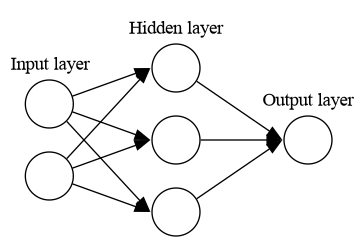
\includegraphics[width=\linewidth]{figures/overview-dense}
		\caption{Overview of dense neural networks.}
		\label{fig:overview-dense}
	\end{subfigure}
	\hfill
	\begin{subfigure}[b]{0.5\linewidth}
		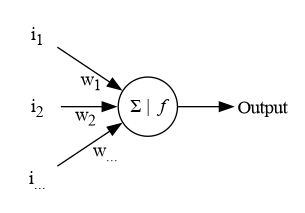
\includegraphics[width=\textwidth, keepaspectratio]{figures/overview-perceptron}
		\caption{Inner workings of an individual perceptron.}
		\label{fig:overview-perceptron}
	\end{subfigure}
\end{figure}

\subsection{Simple Recurrent Neural Network}

Simple Recurrent Neural Networks (SRNN) \cite{new8} are a type of neural network specifically designed to handle sequential data. Unlike traditional feedforward neural networks, SRNNs have the ability to capture temporal dependencies and extract patterns from time sequences of multiple features, adding another dimension to the input data. This temporal aspect is crucial in domains such as time series prediction where the changes in observed values over time are more important than the individual observations themselves \cite{new7}.

The key feature of RNNs is the presence of recurrent connections, which allow information to be passed from one step in the sequence to the next. This enables the network to maintain an internal memory or state, which can be updated and used to influence future predictions. The recurrent connections create a feedback loop that allows the network to consider the entire history of the sequence when making predictions at each step.

Figure \ref{fig:overview-rnn} provides an illustration of how recurrent neural networks work. It shows the flow of information through the network at each time step, with the recurrent connections allowing the network to incorporate information from previous steps.

\begin{figure}[h]
	\centering
	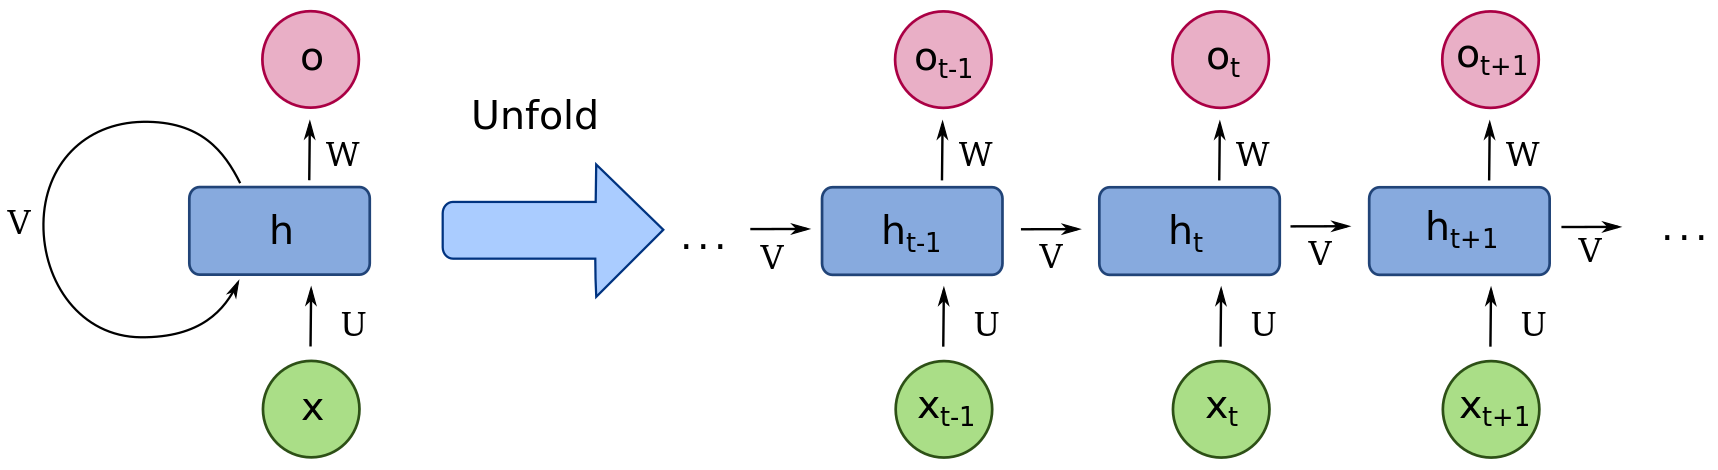
\includegraphics[width=0.8\textwidth, keepaspectratio]{figures/overview-rnn}
	\caption{Overview of a simple RNN layer \cite{fig-srnn}.}
	\label{fig:overview-rnn}
\end{figure}

\subsection{Long Short Term Memory}

SRNNs face challenges in capturing long-term dependencies in sequences. As the sequence length increases, the ability of SRNNs to retain and utilize information from earlier time steps diminishes due to the vanishing gradient problem \cite{rnn-vanishing-gradient}.

The LSTM model was designed to address the vanishing gradient problem more effectively. It consists of three key gates: the forget gate, input gate, and output gate. These gates enable LSTMs to selectively process and store information over sequential data, addressing the vanishing gradient problem. The forget gate determines which information from the previous cell state should be discarded, the input gate decides what new information to store in the cell state, and the output gate regulates what information to output as the hidden state. These gates enable LSTMs to capture long-term dependencies by controlling the flow of information through the memory cell, allowing the model to retain and utilize relevant information while discarding irrelevant portions, which is important for effective sequence learning. An overview of LSTM models is presented in figure \ref{fig:overview-lstm}.

\subsection{Gated Recurrent Unit}

The GRU model is a newer variation of recurrent neural networks. GRUs are similar to LSTMs in that they use a gating mechanisms to selectively update and reset its internal state, allowing it to capture long-term dependencies more efficiently than SRNNs \cite{model-gru}. GRUs have shown to have a similar but slightly lower accuracy as LSTM layers, while being more computationally efficient \cite{gru-lstm-performance}. See figure \ref{fig:overview-gru} for an overview of how GRU models work.

\begin{figure}[h]
	\centering
	\begin{subfigure}[b]{0.45\linewidth}
		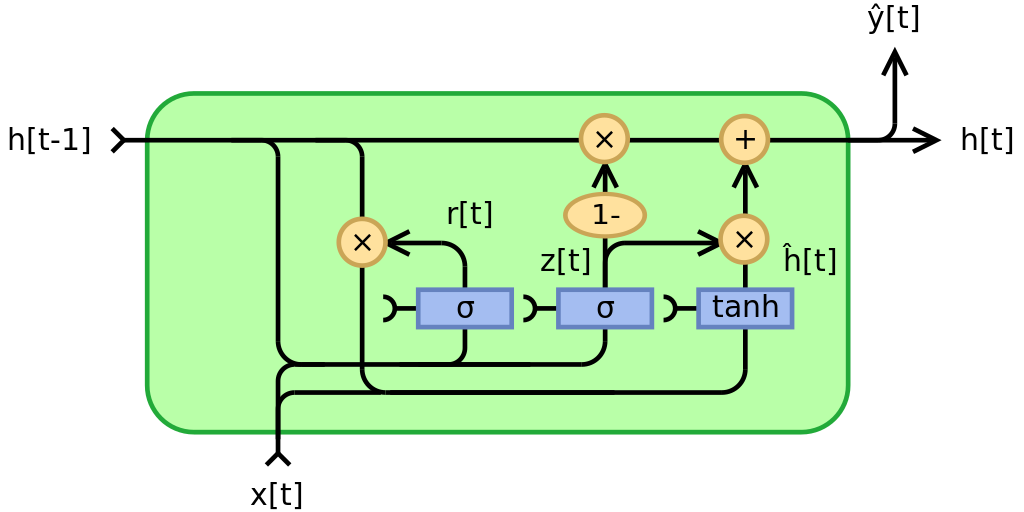
\includegraphics[width=\linewidth, keepaspectratio]{figures/overview-gru}
		\caption{Overview of a GRU layer \cite{fig-gru}.}
		\label{fig:overview-gru}
	\end{subfigure}
	\hfill
	\begin{subfigure}[b]{0.45\linewidth}
		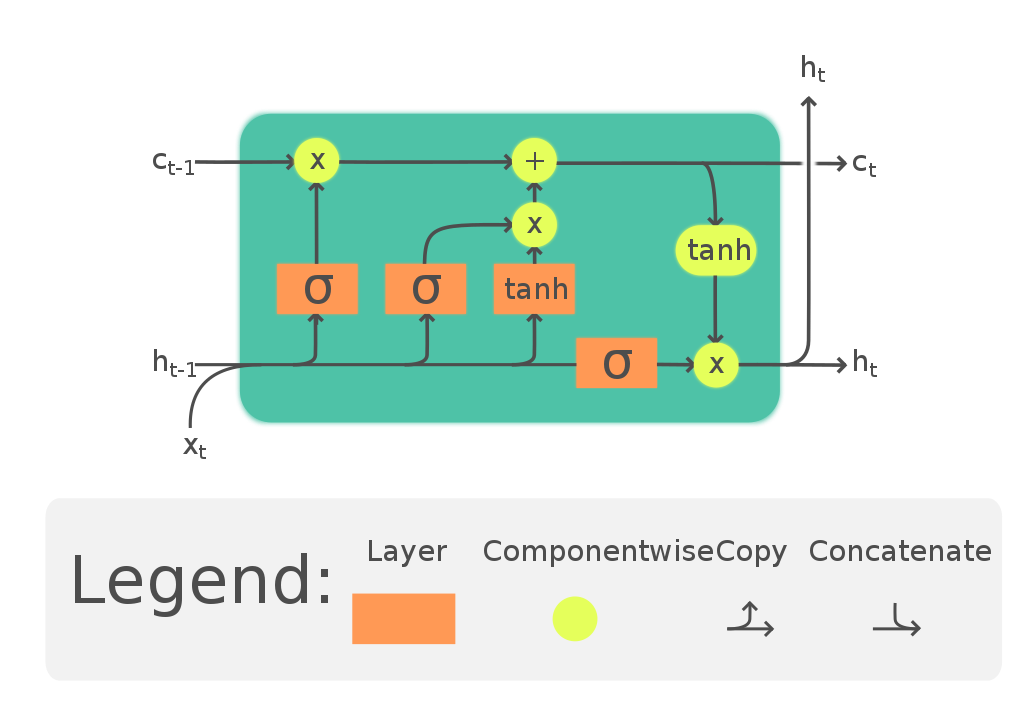
\includegraphics[width=\linewidth, keepaspectratio]{figures/overview-lstm}
		\caption{Overview of a LSTM layer \cite{fig-lstm}.}
		\label{fig:overview-lstm}
	\end{subfigure}
\end{figure}

\section{Optimizing Input Parameters}
\label{sec:method-features}

In order to determine the optimal features for lightning strike prediction, a three-fold strategy was used. The first part involved a manual analysis of both the LIGHT and MESAN data to exclude eventual parameters with a high number of missing values. A visualization of a subset of the LIGHT dataset, serving as the foundation to the binning process, was developed as shown in figure \ref{fig:overview-light}. Secondly, a covariance matrix was constructed to analyze the correlations between parameters. The third part extended the use of the covariance matrix to conduct a Principal Component Analysis.

\subsection{Covariance Matrix}

The correlation analysis was performed using the built-in correlation functionality in R, which uses the Pearson correlation coefficient by default. However, the Pearson correlation coefficient assumes that the underlying data follows a normal distribution. To check for normality among the parameters, the Shapiro-Wilk test was used. The Shapiro-Wilk test is a statistical test that determines if a set of samples follows a normal distribution, and is calculated using equation \ref{eq:shapiro} \cite{shapiro-test}. The results of the test indicate that none of the parameters are normally distributed, meaning an alternative correlation method must be used.

\begin{equation}
	W = {\left(\sum_{i=1}^n a_i x_{(i)}\right)^2 \over \sum_{i=1}^n (x_i-\overline{x})^2}
	\label{eq:shapiro}
\end{equation}

where

\begin{itemize}
	\item $x_{(i)}$ with parentheses enclosing the subscript index $i$ is the $i$th order statistic, i.e., the $i$th-smallest number in the sample (not to be confused with $x_i$).
	\item $\overline{x} = \left( x_1 + \cdots + x_n \right) / n$ is the sample mean.
\end{itemize}

One alternative correlation method is the Spearman's rank correlation coefficient. Unlike the Pearson correlation coefficient, the Spearman's rank correlation coefficient is non-parametric, meaning it does not make any assumptions about the underlying distribution of the data. It is also robust against outliers and can be calculated efficiently. Before calculating the Spearman's rank correlation coefficient, all parameters were normalized.

When training deep neural networks, it is preferable to have fully orthogonal and independent parameters \cite{pca-performance}. This makes the model more efficient as it reduces the amount of input data and calculations required. Therefore, parameters with high correlation may be dropped. However, it is important to note that the statistical tests are not definitive, and it is possible that the removed parameters may prove beneficial.

Based on the covariance matrices presented in section \ref{sec:analysis-mesan-correlation} on page \pageref{sec:analysis-mesan-correlation}, the following parameters were removed due to their high correlation with other, more orthogonal parameters:

\begin{itemize}
	\item Wet-bulb temperature
	\item Cloud base of significant clouds above sea
	\item Total cloud cover
	\item Wind gust
\end{itemize}

\subsection{Principle Component Analysis}

In order to gain a deeper understanding of the MESAN data, a Principal Component Analysis (PCA) was conducted. Humans often struggle to visualize and comprehend data in dimensions higher than three. PCA is a commonly used technique that aims to reduce the dataset into its principal components, a set of orthogonal vectors representing the eigenvalues of the dataset matrix. The primary goal of PCA is to minimize the number of features while retaining the maximum amount of information. Additionally, PCA can be useful for data exploration, providing a more comprehensive understanding of the data. The first principal component (PC1) captures the largest variance in the data. By examining the parameters that have the greatest influence on PC1, it is possible to determine which specific parameters have the most impact on the dataset as a whole.

\section{Hyperparameters Tuning}
\label{sec:method-hypertuning}

A neural network consists of two types of hyperparameters: internal and external. Internal hyperparameters, such as perceptron weights and biases, are automatically optimized during the training process using the training data. On the other hand, external hyperparameters, such as the number of layers, the type and size of each layer, activation functions, and the number of training epochs, need to be manually configured.

The optimization of external hyperparameters is important for achieving good performance in neural networks. Two commonly used methods for optimizing these hyperparameters are random search and grid search. In random search, models are constructed and evaluated with randomly selected hyperparameter values. In grid search, all possible combinations of hyperparameters are evaluated. However, these methods can be computationally inefficient, especially for large search spaces.

Genetic algorithms have shown promising results for hyperparameter tuning compared to random and grid search methods \cite{genetic-algorithms}. Due to the large number of parameters being tested, conducting grid search would be time-consuming, as such in this study a genetic algorithm was used for hyperparameter tuning. The genetic algorithm consists of the following steps:

\begin{enumerate}
	\item An initial population of 100 candidates is generated, where each candidate represents a random combination of hyperparameters.
	\item A fitness value is calculated for each candidate based on its measured accuracy, with an additional penalty for longer training times. The exact formula is presented in equation \ref{eq:fitness}.
	\item The top 10\% best performing candidates survive to create the next generation.
	\item The remaining new candidates are created by sampling two random sequences of the initial candidates, with the probability of selection proportional to their fitness. The candidates in the two sequences are paired and merged to create offspring. Each parameter of the offspring is copied from one of the parents at random, with a 5\% chance of mutation where the parameter is changed to random value.
	\item This process starts anew from step 1.
\end{enumerate}

\begin{equation}
	\text{fitness} = \text{accuracy} - \frac{\text{training time}}{24 000}
	\label{eq:fitness}
\end{equation}

The base architecture of the model used for hyperparameter tuning consists of an input layer followed by a number of recurrent layers, then a number of dense layers, with a final output layer. The purpose of the recurrent layers is to capture the temporal changes in the input data, while the dense layers abstract this knowledge to learn more complex patterns. Note that when evaluating the DNN model, the recurrent layers are replaced with dense layers.

The genetic algorithm was used to determine the optimal values for the following twelve parameters:

\begin{itemize}
	\item Batch size: The number of samples processed in each training iteration.
	\item Optimizer: The algorithm used to update the model's weights during training.
	\item Activation function for the recurrent layers: The function applied to the output of the recurrent layers.
	\item Activation function for the dense layers: The function applied to the output of the dense layers.
	\item Dropout for the recurrent layers: The fraction of input units to drop during training to prevent overfitting.
	\item Dropout for the dense layers: The fraction of input units to drop during training to prevent overfitting.
	\item Number of recurrent layers: The number of recurrent layers in the model.
	\item Number of dense layers: The number of dense layers in the model.
	\item Number of units in the recurrent layers: The number of neurons in each recurrent layer.
	\item Number of units in the dense layers: The number of neurons in each dense layer.
	\item Normalization between recurrent layers: Whether to apply normalization between the recurrent layers.
	\item Normalization between dense layers: Whether to apply normalization between the dense layers.
\end{itemize}

Due to the computational resources required for training hundreds of models through hundreds of generations, only three generations were simulated in this project, making the method similar to a random search. The resulting hyperparameters were copied onto all model types in the final evaluation.

\section{Model Evaluation}

\subsection{Stratified K-Fold Cross-Validation}

When training machine learning models, it is desirable to minimize the impact of randomness and luck. Simply splitting the dataset into two parts, one for training and one for testing, can lead to highly variable results and may not accurately represent the model's performance.

Stratified k-fold cross-validation is a strategy that can be applied to mitigate the impact of randomness. In this study, a $k$ value of $k=10$ has been chosen. The method consists of the following steps:

\begin{enumerate}
	\item Split the data into $k$ different partitions, where each partition contains an equal number of positive and negative samples.
	\item Iterate through the training and evaluation phase $k$ times, with each iteration using a different partition as the test set and the remaining partitions as the training set.
	\item Calculate the evaluation metric for each iteration and set the final evaluation metric as the average of all the test results.
\end{enumerate}

All following metrics were determined using this method.

\subsection{Training Time}

The training time of a deep learning model is an important factor to consider for several reasons. Firstly, it provides an indication of the computational resources required by the model. This is particularly important when deploying the model in real-time applications where fast predictions are necessary. 

Secondly, the training time impacts the development process of the model. During hyperparameter tuning and model development, it is essential to have a manageable training time to iterate and experiment with different configurations effectively. A shorter training time allows for faster experimentation and quicker feedback on the model's performance.

Lastly, the need for retraining the model should also be taken into account. Environmental factors, such as changes in lightning patterns or new geographical locations, may require the model to be updated or retrained periodically. A shorter training time facilitates this process, enabling the model to adapt to new data and maintain its accuracy over time.

\subsection{F1 Score}

The F1 score is a metric commonly used in machine learning evaluation as it provides a more comprehensive metric than simple accuracy. It is a compound metric derived multiple independent metrics.

\paragraph{Accuracy:}
Accuracy is the most prevalent and simplest type of machine learning metric. It gives an indication of the frequency of correct predictions made by the model. It is calculated as the ratio of the number of correct predictions to the total number of predictions made by the model. The formula for accuracy is shown in equation \ref{eq:metric-accuracy}. 

\begin{equation}
	\text{accuracy} = \frac{\text{correct predictions}}{\text{total predictions}}
	\label{eq:metric-accuracy}
\end{equation}

\paragraph{Binary Accuracy:}
A critical issue arises when using accuracy on binary classification models. The model outputs a probability that represents how likely a sample belongs to a class, rather than the actual class itself. Because of this, using simple accuracy would constantly result in 0\% accuracy as very few of the predictions match the label exactly. To accommodate for this, binary accuracy rounds the output of the model to the closest class before evaluating, making it a practically feasible metric.

\paragraph{Precision \& Recall:}
\label{sec:precision-recall}
While binary accuracy is a commonly used metric for evaluating model performance, it may not provide a complete picture, especially when dealing with imbalanced testing data. To address this, two additional metrics, precision and recall, are introduced.

Precision measures the accuracy of the model's positive predictions. It answers the question: "Out of all samples predicted as positive, how many were actually positive?". A high precision indicates a low rate of false positives. The formula for calculating precision is shown in equation \ref{eq:precision}.

Recall, on the other hand, measures the model's ability to correctly identify all positive samples. It answers the question: "Out of all actual positive samples, how many were correctly predicted?". A high recall indicates that the model is effective at identifying positive samples, but it may have a higher rate of false negatives. The formula for calculating precision is shown in equation \ref{eq:recall}.

\begin{minipage}{0.5\linewidth}
	\begin{equation}
		\frac{\text{true positives}}{\text{true positives} + \text{false positives}}
		\label{eq:precision}
	\end{equation}
\end{minipage}
\begin{minipage}{0.5\linewidth}
	\begin{equation}
		\frac{\text{true positives}}{\text{true positives} + \text{false negatives}}
		\label{eq:recall}
	\end{equation}
\end{minipage}

\paragraph{F1-Score:}
Finally, the F1-score is a metric used to measure the performance of a classification model. It is the harmonic mean of precision and recall. The F1-score combines these two metrics to provide a single value that represents the balance between precision and recall, and can thus be used for model comparison. It ranges from 0 to 1, with 1 being the best possible score. A higher F1-score indicates a better overall performance of the classification model. Equation \ref{eq:f1-score} shows how the f1-score is calculated.

\begin{equation}
	2 \frac{precision \cdot recall}{precision + recall}
	\label{eq:f1-score}
\end{equation}

\subsection{Mean Absolute Error}

The mean absolute error (MAE) metric is used to measure the average level of confidence the model has in its predictions. A lower value indicates a higher confidence, as the individual predictions deviate from the true value by this average amount. While being an uncommon metric as it is the accuracy that count, it can be a useful metric when comparing models with very similar accuracy.

\subsection{Wilson Score}

The Wilson Score is a statistical method used to estimate the confidence interval for binary accuracy. It provides a range of values within which the true accuracy of the model is likely to fall, with a chosen confidence level of 95\% used in this study. The Wilson Score helps assess the accuracy of the model.

\section{Time frames}

In order to assess the performance of the models across different time frames, two additional evaluation factors are introduced: \textit{lookback} and \textit{lookahead}.

The lookback refers to the size of the temporal dimension of each feature sequence. A higher lookback value increases the time window, while a lower value decreases it. For instance, a lookback of 24 implies that the model can utilize one day of data, with an hourly frequency, as input. 

On the other hand, the lookahead signifies the size of the window within which the model is expected to make predictions. A lookahead of 24 means that the model should predict the occurrence of a lightning strike within a 24-hour period, while a lookahead of 1 means predicting if a lightning strike will happen within the next hour.

In order to comprehensively evaluate the models, various combinations of lookback and lookahead values are explored. This allows for analyzing the impact of different time frames on the performance of the DL models. By considering a range of lookback and lookahead values, it is possible to gain insights into the optimal time window for predicting lightning strikes. Additionally, by examining the effect of different time frames on the model's accuracy, it is possible to determine the most suitable time frame for practical applications. Due to the limited number of available observations however, the largest combination of lookback + lookahead that can be used cannot exceed 73 hours.

Furthermore, it is worth mentioning that the choice of lookback and lookahead values should be guided by the specific requirements of the application. For instance, if the goal is to provide real-time lightning strike predictions for immediate safety measures, a shorter lookahead period, such as 1 hour, may be more appropriate. On the other hand, if the objective is to forecast lightning strikes for longer-term planning, a larger lookahead period, such as 24 hours, could be more beneficial.

\subsection{Data Structuring}

Before training the model, the data needs to be restructured based on the lookback and lookahead parameters. Changing the lookback is straightforward, as it involves adjusting the number of observations in the lookback sequence leading up to the lightning strike. However, changing the lookahead is more complex.

When increasing the lookahead to a value greater than 1, a lookahead sequence needs to be created where the lightning strike can occur at any time point, not just the first time point. This requires shifting the lookahead sequence backwards by a random amount, which renders a portion of the lookback sequence unusable. Consider figure \ref{fig:lookahead-one}, where the lookback sequence $X$ leading up to lightning strike $Y$ has to be shifted to allow $Y$ to occur at any point in the lookahead sequence.

\begin{figure}[h]
	\centering
	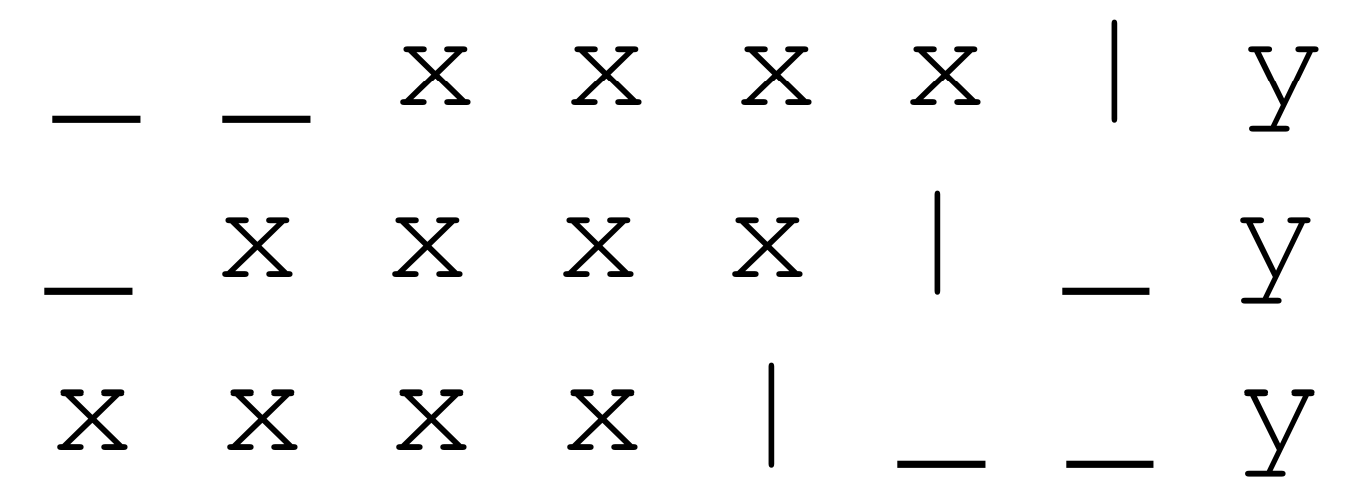
\includegraphics[width=0.3\textwidth, keepaspectratio]{figures/lookahead-one}
	\caption{Illustration of lookahead shifting.}
	\label{fig:lookahead-one}
\end{figure}

Furthermore, within the newly created lookahead sequence, another independent lightning strike may have occurred, either at the same location or a nearby one. Therefore, the binning method used previously (see Section \ref{sec:preprocessing-light-binning} on page \pageref{sec:preprocessing-light-binning}) needs to be reapplied to every other lightning strike in the LIGHT dataset. If another lightning strike has occurred within the lookahead sequence, the label is changed to positive, regardless of its previous class. Consider figure \ref{fig:lookahead-two}, where a negative samples becomes positive after lightning strike $Z$ gets included in the lookahead.

\begin{figure}[h]
	\centering
	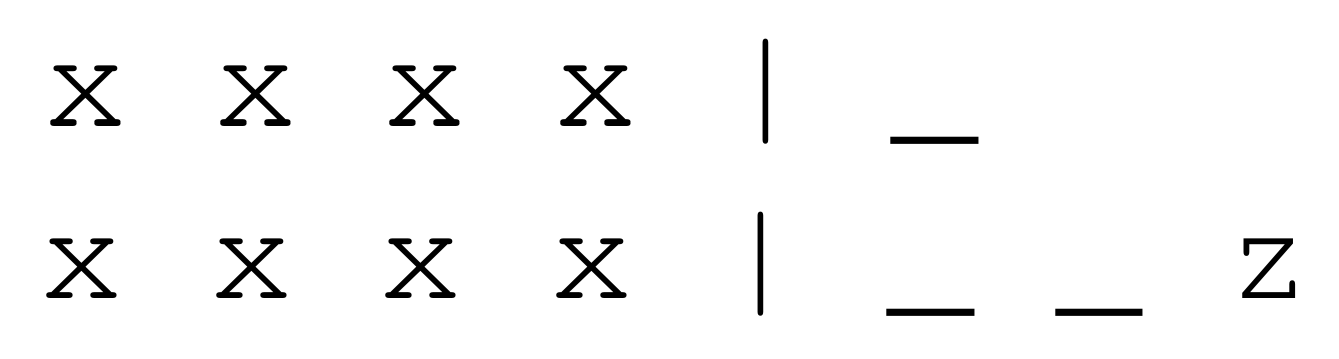
\includegraphics[width=0.3\textwidth, keepaspectratio]{figures/lookahead-two}
	\caption{An independent lightning strike occurring within the lookahead sequence.}
	\label{fig:lookahead-two}
\end{figure}

When changing the distribution of labels, it is important to again consider class skewness. After restructuring the dataset to accommodate the lookahead parameter, it is likely that the dataset is biased towards a positive label. At this stage, it is not feasible to regenerate or change the dataset. Therefore, class weights are used as a last resort. The class weighting mechanism examines the restructured dataset and calculates the ratio between positive and negative samples. This ratio is then used to adjust the weight or importance of each label in that class during training.

